\documentclass[12pt,a4paper,oneside]{article}

\usepackage[utf8]{inputenc}
\usepackage[T1]{fontenc}
\usepackage[french]{babel}
\usepackage{amssymb}
\usepackage{amsmath}
\usepackage{graphicx}
\usepackage{float}
\usepackage{mathtools}


\author{Matteo Besançon}
\title {Préparation examens outils formels}
\date{\today}
\begin{document}
	\maketitle

\section{Formalisme RdP}
	\subsubsection*{1. Définition formelle de la structure des RdP (syntaxe)}
		\begin{description}
			\item [P] Places (Rond)
			\item [T] Transitions (Rectangle)
			\item [ ] Jeton (point noir)
		\end{description}

		Un réseau R est un quadruplet R

		$$R = (P,T, Entree, Sortie)$$

		Pour $p \in P$ et $t \in T$ si :
		\begin{itemize}
			\item $k = Entree(p,t) > 0$ $p$ est une place d'entrée de $t$ et $t$ est une place de sortie de $p$
			\item $k = Sortie(p,t) > 0$ $p$ est une place de sortie de $t$ et $t$ est une place d'entrée de $p$
		\end{itemize}

		On a les représentations matricielles suivantes :

		\begin{figure}[H]
			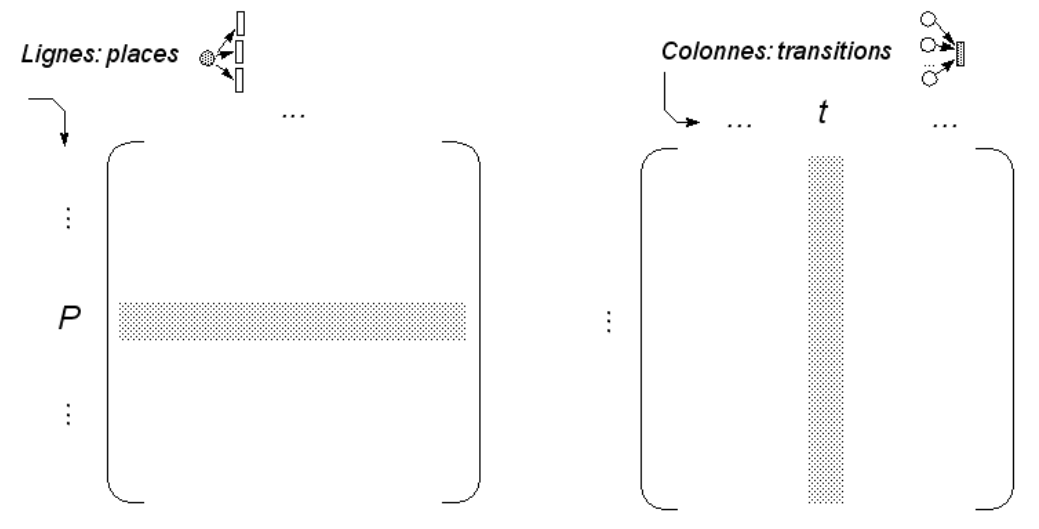
\includegraphics[scale = 0.4]{./img/entree.png}
			\centering
			\caption{Matrice d'entrée et de sortie}
			\label{entreeSortie}
		\end{figure}

		Par exemple avec le RdP suivant :

		\begin{figure}[h]
			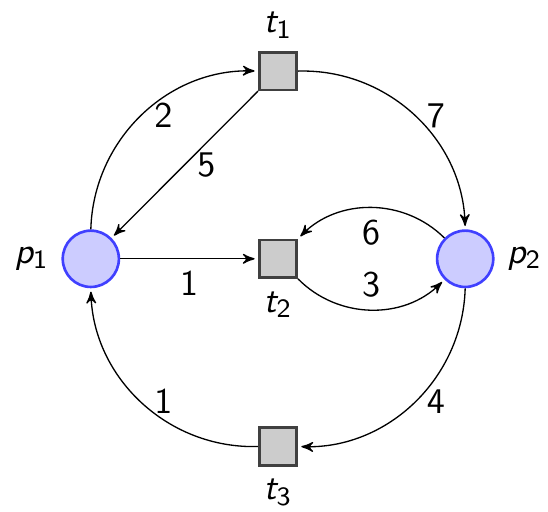
\includegraphics[scale = 0.5]{./img/exrdp.png}
			\centering
			\caption{RdP d'exemple}
			\label{exrdp}
		\end{figure}

		On a donc les matrices suivantes :
		$$Entree = \begin{bmatrix}
			2 & 1 & 0 \\
			0 & 6 & 4
		\end{bmatrix}
		Sortie = \begin{bmatrix}
			5 & 0 & 1 \\
			7 & 3 & 0
		\end{bmatrix}$$

		L'état d'un RdP est appelé un marquage $M:P\to \mathbb{N}$ souvent le marquage initial est noté $M_0$

		Pour la figure \ref{exrdp} on a la matrice de marquage:
		$$M = \begin{pmatrix}
			2\\
			3
		\end{pmatrix}$$
	\subsubsection*{2. Définition formelle des règles de franchissabilité des transitions (sémantique)}
		Y a un jeton et paf plus de jeton !!

	\subsubsection*{3. Utilisation de l'algèbre linéaire pour définir la franchissabilité des transitions}

	Une transition $t$ est franchissable (tirable) si :
	$$\forall p \in P,\ M(p) \geq Entree(p,t)$$
	par exemple pour la figure \ref{exrdp} $t_1$ est tirable et $t_3$ ne l'est pas.

	Après avoir tiré la transition $t$ on a :
	$$\forall p \in P,\ M'(p) = M(p) - Entree(p,t) + Sortie(p,t)$$

	On a la notation $M \xrightarrow[]{t} M'$

	On note $C$ la matrice d'incidence du réseau définie par
	$$\forall p \in P,\ \forall t \in t,\ C(p,t) = Sortie(p,t) - Entree(p,t)$$

	donc
	$$M' = M + C(\dots,t)$$

	Si on reprends l'expemple de la figure \ref{exrdp}
	$$C = \begin{bmatrix}
		3 & -1 & 1 \\
		7 & -3 & -4
	\end{bmatrix}$$

	Et donc si on tire $t_1$
	$$M' = M + C(\dots,t_1) =
	\begin{pmatrix}
		2\\
		3
	\end{pmatrix}
	+
	\begin{bmatrix}
		3 & -1 & 1 \\
		7 & -3 & -4
	\end{bmatrix}
	\begin{pmatrix}
		1\\
		0\\
		0
	\end{pmatrix}
	=
	\begin{pmatrix}
		5\\
		10
	\end{pmatrix}
	$$

	\subsubsection*{4. Propriétés des séquences de franchissements, vecteur caractéristique et équation fondamentale}

		On a la séquece de transition $T_1T_2$ On peut écrire
		$$s = T_1T_2$$
		$$M_0 \xrightarrow[]{s} M_2$$

		$\overline{s}$ est le vecteur caractéristique de la séquence $s$ tel que
		$$\overline{s}: T \rightarrow \mathbb{N}$$
		$$\overline{s}(t) = \textrm{le nombre d'occurences de t dans } s$$

		En prenant l'exemple de la figure \ref{exrdp} avec la séquence $t_1t_2t_2t_3t_1$ on a le vecteur caractéristique suivant :
		$$\overline{s} = \begin{pmatrix}
			2\\
			2\\
			1
		\end{pmatrix}$$

		On a les propriétés suivantes
		$$s = s_1 \cdot s_2$$
		$$\overline{s} = \overline{s_1} + \overline{s_2}$$

		Pour $M \xrightarrow[]{s} M'$ on a :
		$$M' = M + C \cdot \overline{s}$$
	 	qui est \textbf{l'équation fondamentale}.

\section{Propriétés des RdP}
	\subsubsection*{5. Monotonie et répétitivité des séquences de transitions}

		Dénfinition :
		$$M_a \leq M_b \textrm{ si } \forall p \in P M_a(p) \leq M_2(p)$$

		Une séquence est dite \textbf{monotone} si
		$$M_1 \xrightarrow[]{s} M \textrm{ et } M_1 \leq M_2$$

		Alors
		$$M_2 \xrightarrow[]{s} M + (M_2 - M_1)$$

		Une séquence est dite \textbf{répétitive} si
		$$\forall M \textrm{ t.q. } M \xrightarrow[]{s}$$

		Alors
		$$\forall n \in \mathbb{N^+}, M \xrightarrow[]{s^n}$$

	\subsubsection*{6. "Bornitude" et répétitivité des séquences de transitions}

		Un marquage $M'$ est \textit{accessible} si
		$$\exists s \in T^* \textrm{ t.q. } M \xrightarrow[]{s} M'$$

		L'ensemble des marquages accessibles dans un Reseau $R$ depuis $M$ est noté $A(R,M)$

		Une place $p$ du réseau $(R, M_0)$ est \textbf{k-bornée} si
		$$\forall M \in A(R, M_0),\ M(p) \leq k$$

		Une séquence répétitive est croissante pour $p$ si :
		$$\forall M, M' \in A(R, M_0) \textrm{ t.q. } M \xrightarrow[]{s} M'$$

		Alors
		$$M(p) < M'(p)$$

		Un réseau $(R, M_0)$ est \textbf{non borné} si et seulement si
		\begin{itemize}
			\item $\exists s$ répétitive croissante pour $p$
			\item $\exists M \in A(R, M_0)$
		\end{itemize}
		Tel que $M \xrightarrow[]{s}$
	\subsubsection*{7. Monotonicité, quasi-vivacité, vivacité et blocage}

		Une transition $t$ est dite \textbf{quasi-vivante} pour $M_0$ si et seulement si
		$$\exists M \in A(R,M_0),\ M \xrightarrow[]{t}$$

		Un réseau est quasi-vivant si
		$$\forall t \in T,\ t \textrm{ est quasi-vivant}$$

		Une transition $t$ est dite \textbf{vivante} si et seulement si
		$$\forall M \in A(R,M_0), t \textrm{ est quasi-vivant pour } M$$

		Un réseau est vivant si
		$$\forall t \in T,\ t \textrm{ est vivant}$$

		\textbf{Attention} la vivacité n'est pas monotone contrairement à la quasi-vivacité

		Une séquence répétitive $s$ est dite complète si
		$$\forall t \in T,\ \overline{s}(t) \geq 1$$

		On a donc la relation suivante :
		$$(R, M_0) \textrm{ vivant } \iff
		\forall M \in A(R,M_0),\
		\exists M' \in A(R,M),\
		\exists s \in T^* \textrm{ complète t.q. }
		M' \xrightarrow[]{s}$$

		Un marquage puit est un marquage pour le quel aucune transition n'est tirable
		$$Puit(M) \iff \nexists t \in T \textrm{ t.q. } M \xrightarrow[]{t}$$

		Un reseau $(R,M_0)$ est sans blocage si
		$$\forall M \in A(R,M_0),\ \neg Puit(M)$$

	\subsubsection*{8. État d'accueuil, réversibilité, répétitivité, consistance}

		Un réseau a un \textbf{marquage d'accueuil} $M_a$ pour un marquage initial $M_0$ si
		$$\forall M_i \in A(R,M_0),\ \exists s \in T^* \textrm{ t.q. } M_i \xrightarrow[]{s} M_a$$

		Un rdP est \textbf{réinitialisable (ou réversible)} pour un marquage initial $M_0$ si $M_0$ est un état d'accueil.

		Un rdP est \textbf{répétitif} s'il existe un marquage initial $M_0$ et une séquence $s$ franchissable telle que chaque transition apparait un nombre illimité de fois.

		Un réseau est \textbf{consistant} si il exite un marquage initial $M_0$ et $s$ contenant au moins une fois toute les transitions tels que
		$$M_0 \xrightarrow[]{s} M_0$$

\section{Vérification des propriétés}
	\subsubsection*{9. Définition du graphe de marquages, définition du graphe de couverture}


\end{document}
